Működés közbeni tesztelésre az FPGA-ba beépített ILA (Integrated Logic Analyser) volt felhasználva.

\subsection{WS2813\_Driver}

Ennél a modulnál szükség van egy 24 bit-es bementre. Mivel annyi kapcsoló nem található a választott FPGA lapon, ezért a modul le lett egyszerűsítve, a tesztelés megkönnyebítéséért. 
24 bemenet helyett csak 4 lett felhasználva, ezek be is lettek konfigurálva az fpga négy kapcsolójára.

Ezen kívül a done és a d\_out jelek egy-egy LED-re lettek kötve. A d\_out jelnek ledre való kötése később értelmetlennek bizonyult, mivel olyan gyors a váltakozás magas feszűltésgről alacsony feszűltségre
a küldés során, hogy a LED fel sem gyúl.
A rendszer működés közbeni teszteléséhez szükséges volt egy trigger definiálásához: amikor a d\_out jel 1-esre vált, akkor kezdődjön a mintavételezés. Ez lehetővé teszi, hogy a küldés kezdetétől legyen a mintavételezés.

FPGA állapota 0000 küldése esetén:

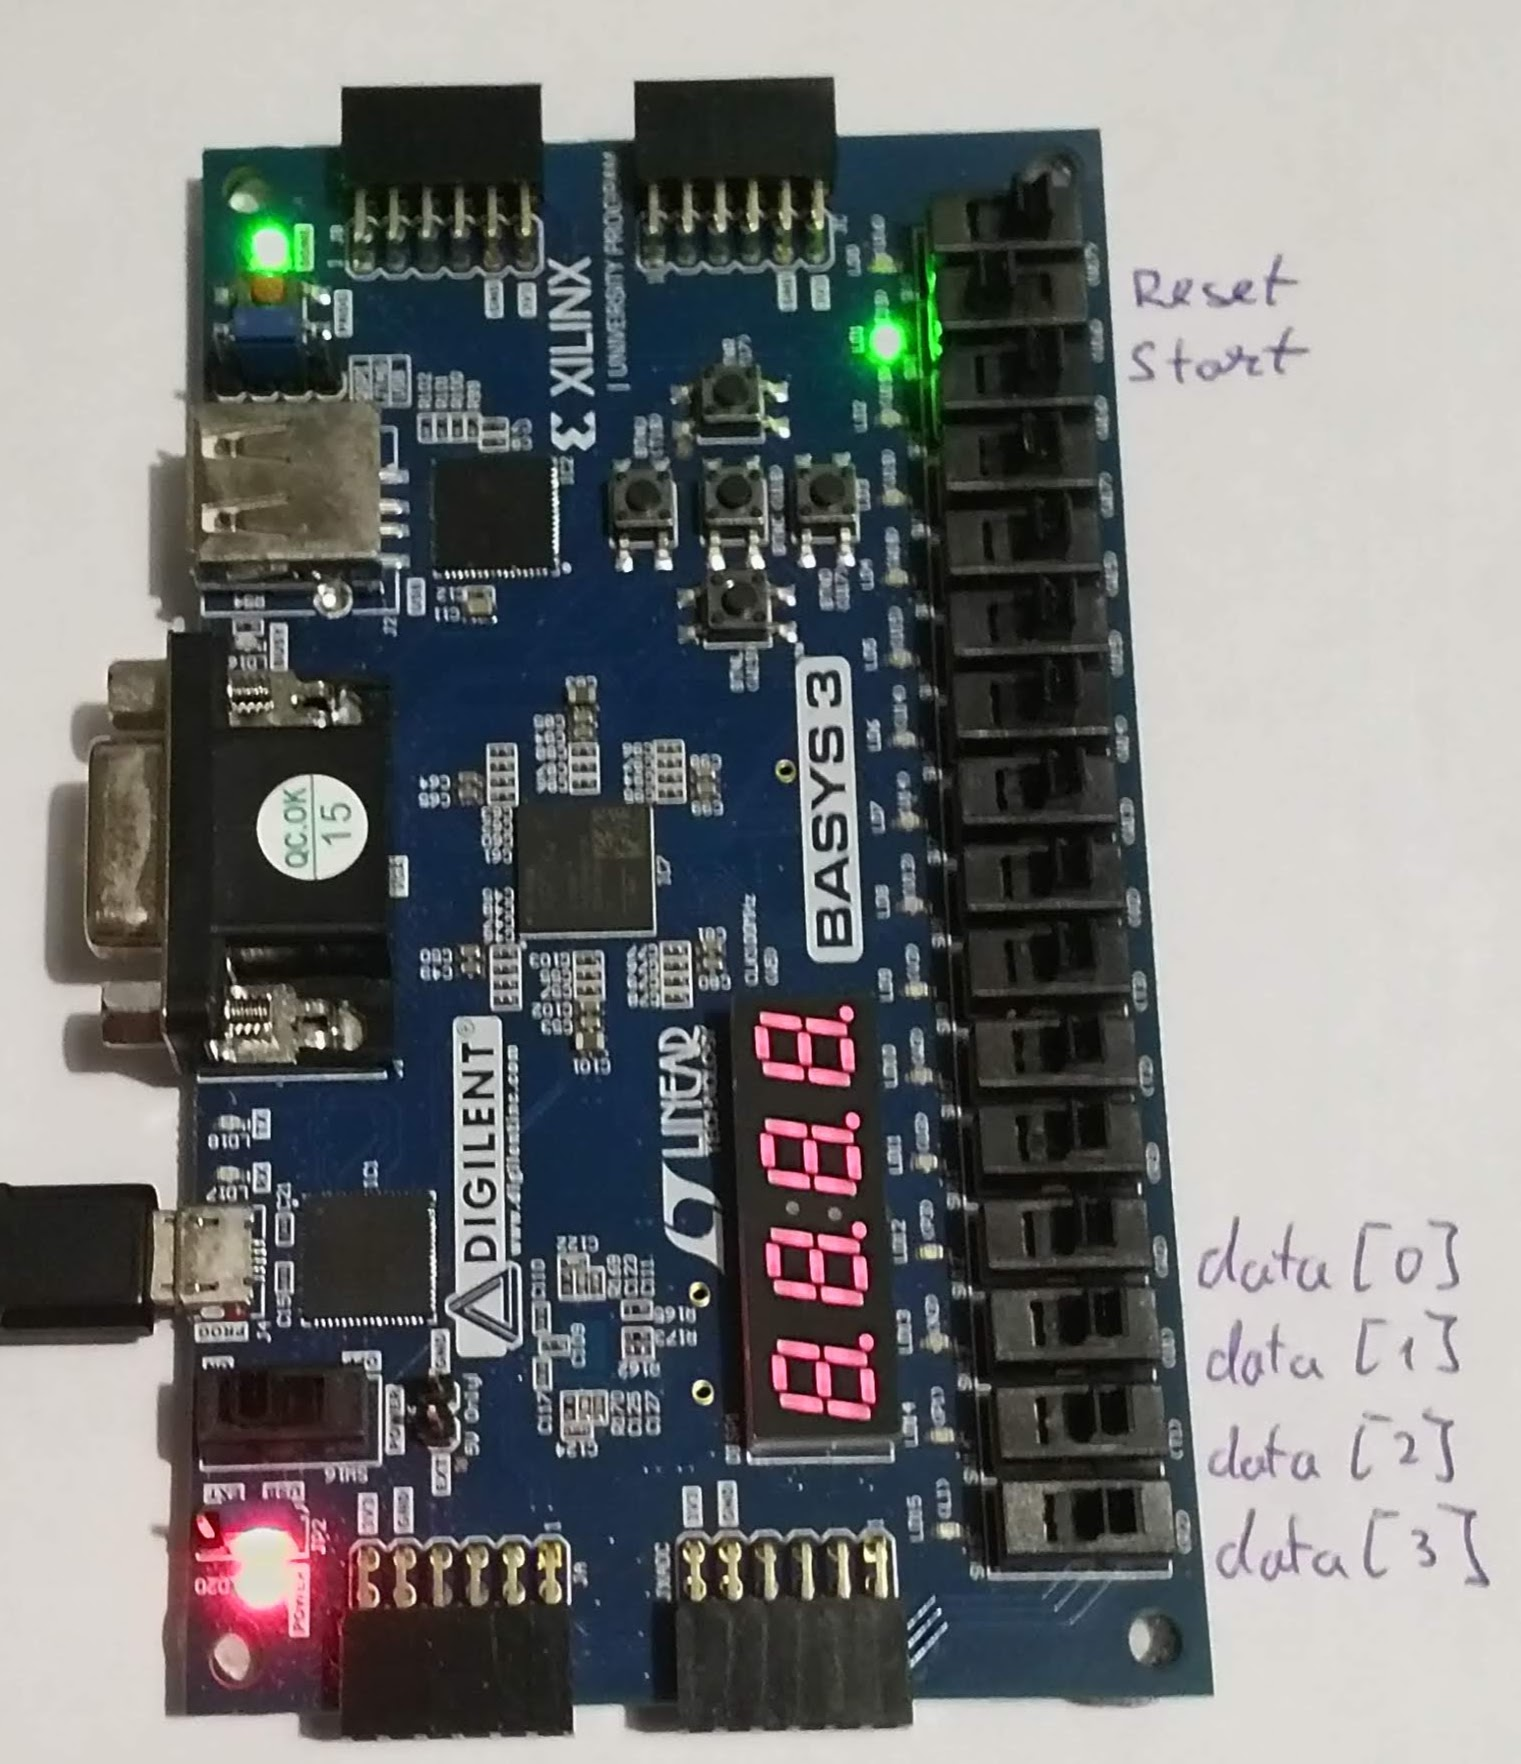
\includegraphics[scale=0.2]{fpga_0000.jpg}

Jelek 0000 küldése esetén:

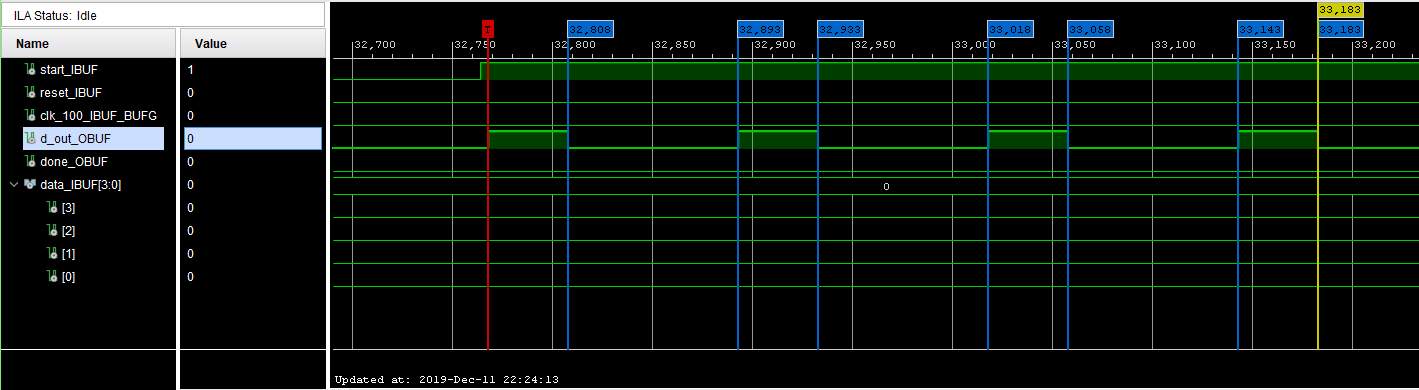
\includegraphics[scale=0.43]{ila_0000.PNG}

Amint az FPGA-ról és a jelanalizálása közben is látható, az elküldött adat 0000. Ugyanakkor az is látható, hogy a d\_out jel annyi időt van magas és alacsony feszűltségen, amennyit a protokoll megkövetel.
Ezen a példán nem látszik, hogy a küldés az MSB-től (Most Significant Bit) lenne elkezdve. Ennek demonstrálásához egy "asszimetrikus" adat szükséges, mint például: 0010

FGPA állapota 0010 küldése esetén:

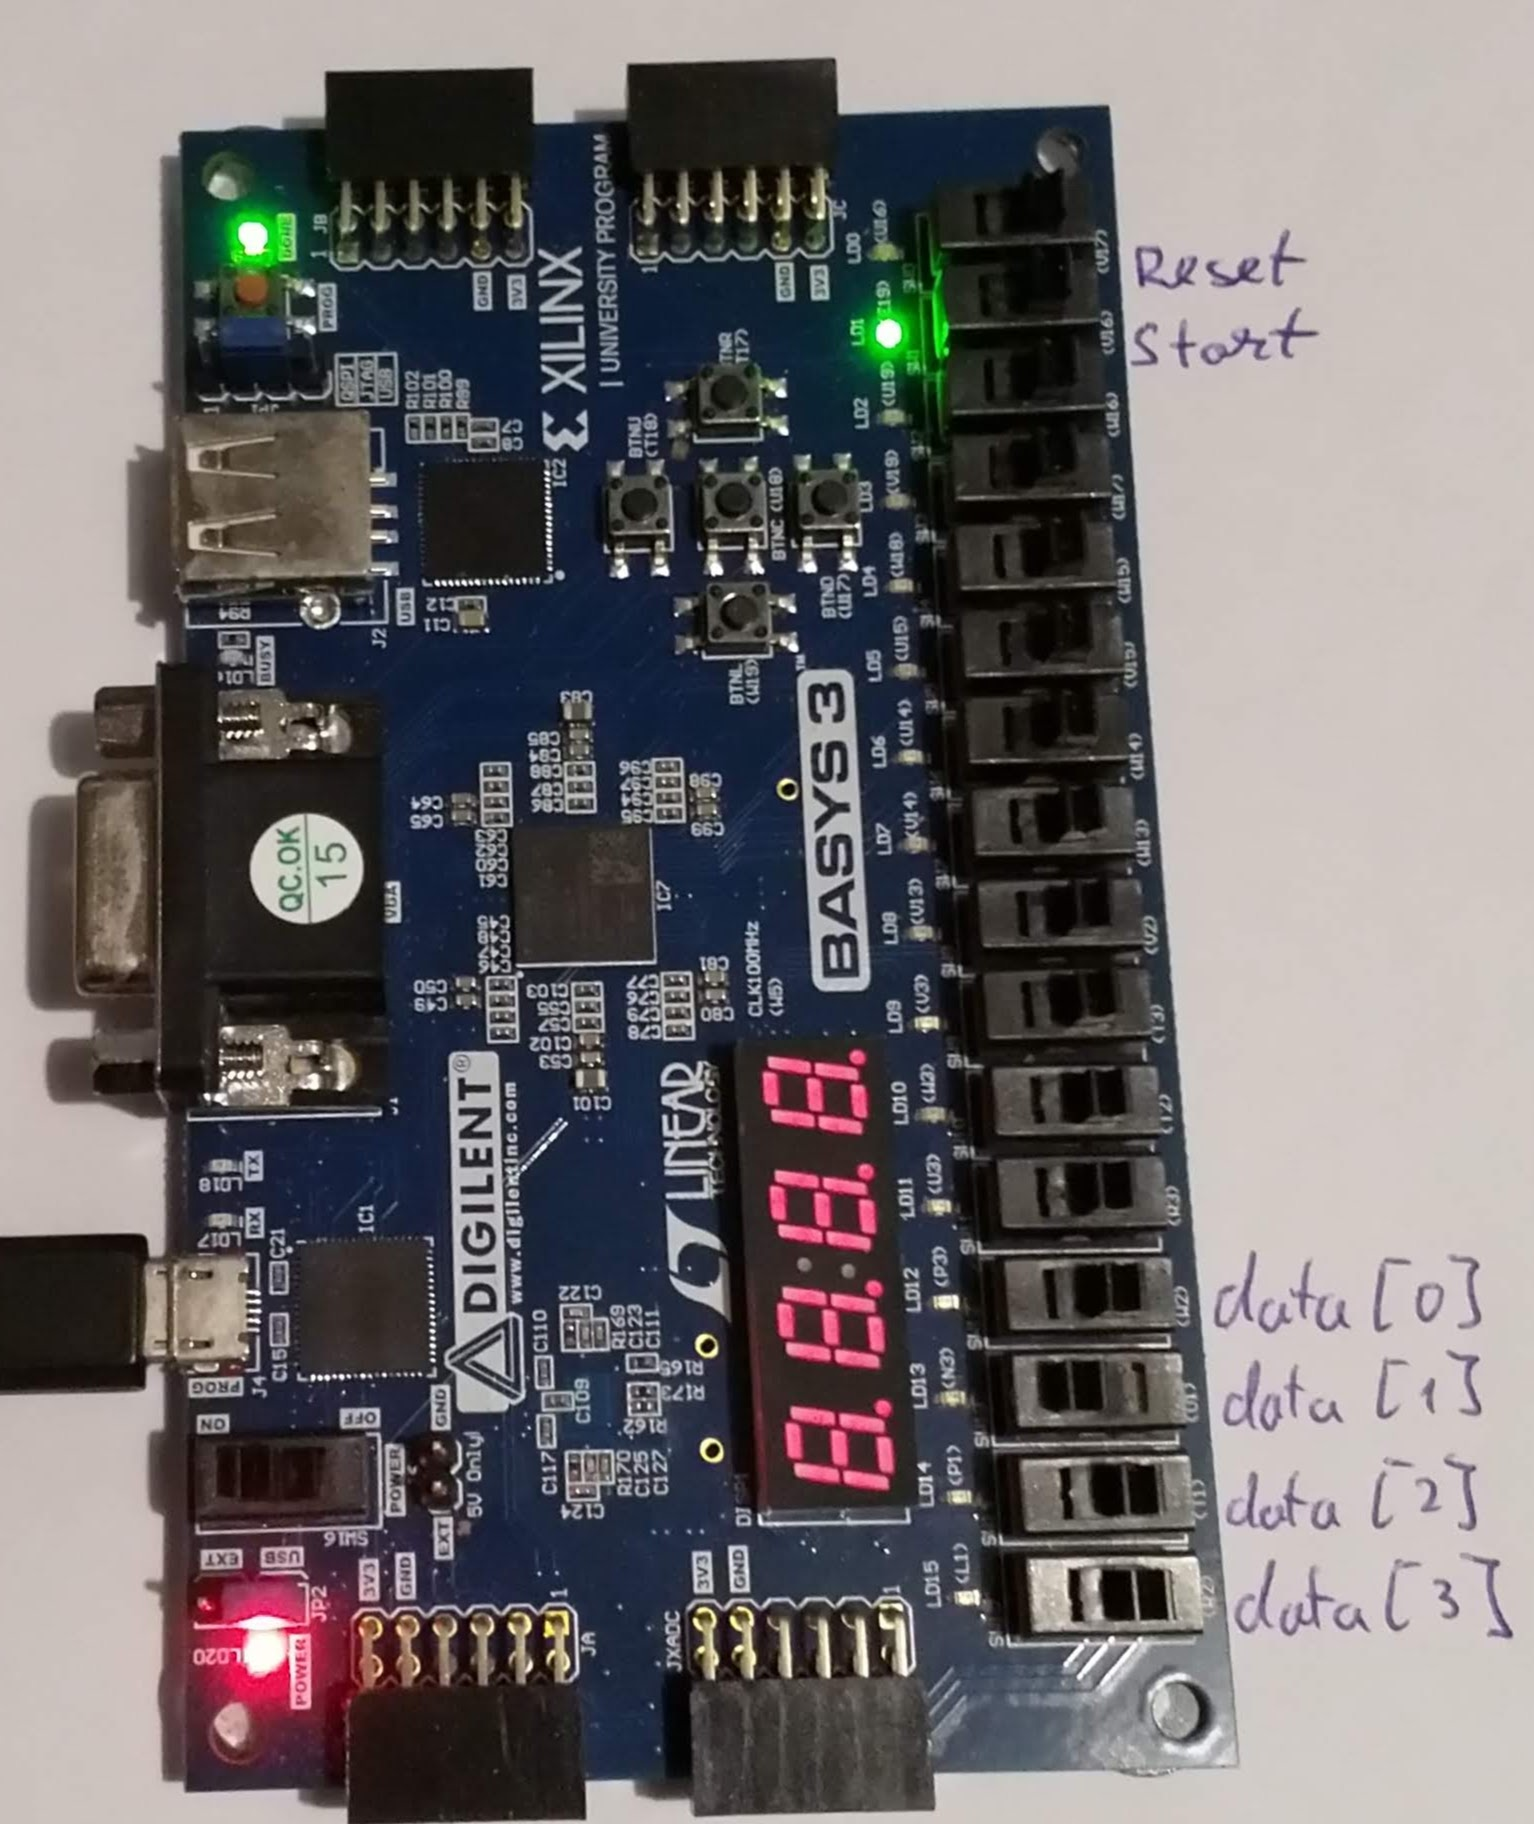
\includegraphics[scale=0.2]{fpga_0010.jpg}

Jelek 0010 küldése esetén:

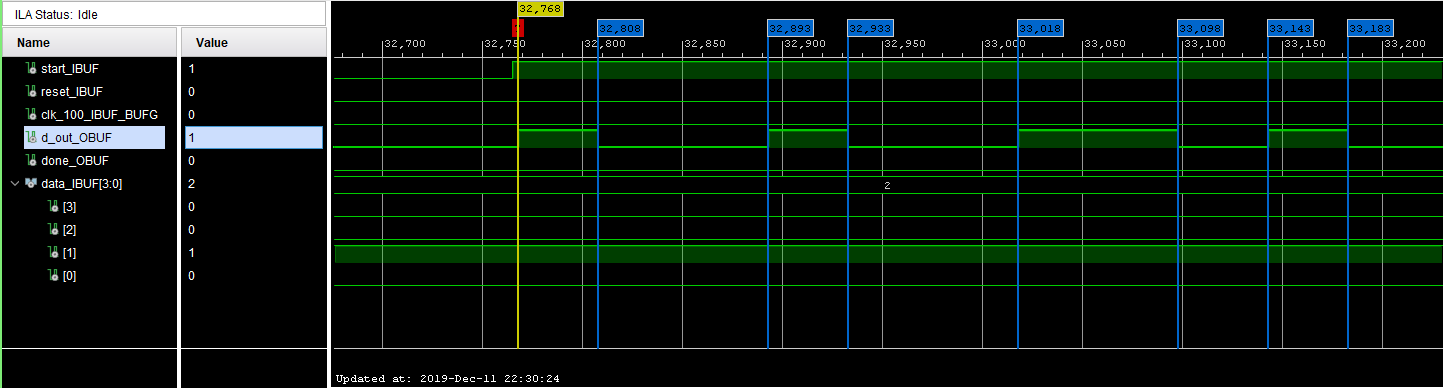
\includegraphics[scale=0.40]{ila_0010.PNG}

Látható, hogy a küldés az MSB-től van elkezdve. Ugyanakkor az is megfigyelhető, hogy a WS2813 protokollja be van tartva.

\subsection{Teljes rendszer működés közbeni tesztelése}

TODO